\thispagestyle{empty}
\begin{tikzpicture}[remember picture,overlay]
  \node[anchor=center] at (current page.center) {%
    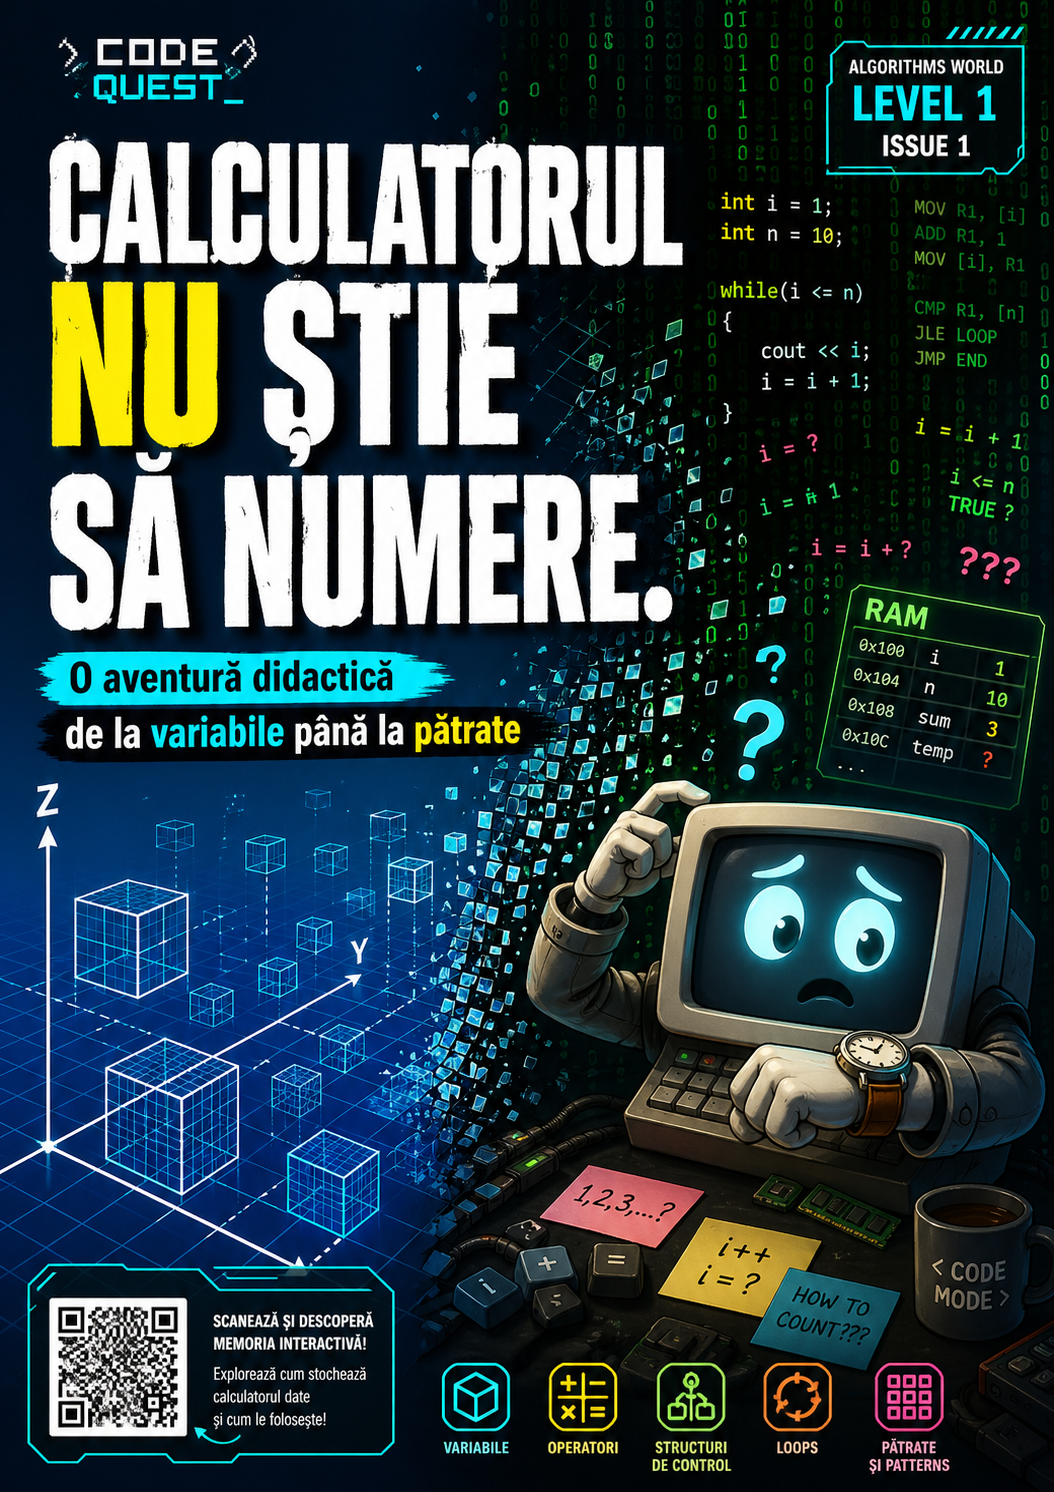
\includegraphics[width=\paperwidth,height=\paperheight]{../cover/cover.png}%
  };
\end{tikzpicture}
\null
\clearpage

\SetPageTheme{paper}
\color{black}
\thispagestyle{empty}
\null
\clearpage

\SetPageTheme{paper}
\color{black}
\thispagestyle{empty}
\begin{center}
{\Huge\bfseries \IssueTitle}\par
\vspace{0.6em}
{\Large \IssueSubtitle}\par
\vspace{1.4em}
\rule{0.72\linewidth}{0.8pt}\par
\vspace{1.2em}
{\large Numarul 1 din colectia \IssueCollection}\par
\vspace{0.6em}
{\normalsize Nivel recomandat: clasele V--VIII}\par
\vspace{0.4em}
{\normalsize Domeniu: algoritmica, logica, jocuri si reprezentare pe grila}\par
\end{center}

\vspace{1.8em}

\begin{tcolorbox}[colback=white,colframe=black!55,boxrule=0.7pt,arc=1.5mm]
\small
\textbf{Cum folosim acest auxiliar}

Se lucreaza cu creionul in mana. Paginile nu sunt doar pentru citit, ci pentru urmarit stari, completat tabele, trasat output-uri si descris in cuvinte ce se intampla in cod.
\end{tcolorbox}

\vspace{0.8em}

\begin{tcolorbox}[colback=white,colframe=black!55,boxrule=0.7pt,arc=1.5mm]
\small
\textbf{Ce vei intalni}
\begin{itemize}
\item pagini de idee, in care o notiune noua este explicata pe scurt si clar;
\item pagini de exercitiu, in care urmaresti transformari si completezi lipsurile;
\item pagini cu QR pentru simulatoare si experimente Blockly;
\item o provocare finala in care toate ideile se leaga intr-un joc.
\end{itemize}
\end{tcolorbox}

\vfill
\begin{center}
\small Acest numar merge de la memorie si numarare la decizie, repetitie, grile si jocuri.
\end{center}
\clearpage

\SetPageTheme{paper}
\color{black}
\thispagestyle{empty}
\begin{center}
{\Huge\bfseries Cuprins}\par
\vspace{1.4em}
\end{center}

\begin{tabularx}{\linewidth}{@{}Xr@{}}
Calculatorul nu stie sa numere: intrarea in poveste & 5 \\
Variabile si memorie & 8 \\
Operatori aritmetici & 13 \\
Evaluare si recapitulare & 18 \\
Structuri de control: harta mare & 20 \\
Structura \texttt{daca} & 24 \\
Structura \texttt{cat timp} & 30 \\
Structura \texttt{pentru} & 36 \\
Evaluare FizzBuzz & 42 \\
Structuri imbricate, Pong si TicTacToe & 46 \\
Provocarea redactiei & 62 \\
\end{tabularx}

\vspace{1.5em}

\begin{tcolorbox}[colback=white,colframe=black!55,boxrule=0.7pt,arc=1.5mm]
\small
\textbf{Observatie}

Numerele de pagina sunt orientative pentru aceasta editie si pot suferi mici deplasari dupa ultimele ajustari grafice.
\end{tcolorbox}

\clearpage

\SetPageTheme{paper}
\color{black}
\thispagestyle{empty}
\begin{center}
{\Huge\bfseries Inainte sa intram in lectii}\par
\vspace{0.8em}
{\large Firul pe care il vom urmari de la prima pagina pana la jocul final}\par
\end{center}

\vspace{1.2em}

\begin{tcolorbox}[colback=white,colframe=black!60,boxrule=0.8pt,arc=1.5mm]
\small
Calculatorul nu stie sa numere, sa aleaga sau sa deseneze singur. Tot ce poate face este sa tina minte valori si sa aplice reguli foarte precise. De aici porneste toata editia aceasta.

Mai intai vom vedea cum tine minte starea unui joc: vieti, scor, pozitie, energie, chei. Apoi vom vedea cum acea stare se modifica prin operatii simple. Dupa aceea intram in structurile de control, adica in locul in care programul incepe sa aleaga si sa repete. La final, toate ideile se strang intr-o grila, intr-un mic model de Pong si intr-o provocare de TicTacToe.
\end{tcolorbox}

\vspace{0.8em}

\begin{tcolorbox}[colback=white,colframe=black!60,boxrule=0.8pt,arc=1.5mm]
\small
\textbf{Intrebarea care ramane in fundal}

La aproape fiecare pagina merita sa ne intrebam doua lucruri:
\begin{enumerate}
\item ce stare tine minte calculatorul acum;
\item ce regula o schimba.
\end{enumerate}

Daca raspunsul este clar, inseamna ca si logica programului este clara.
\end{tcolorbox}

\vspace{0.8em}

\begin{tcolorbox}[colback=white,colframe=black!60,boxrule=0.8pt,arc=1.5mm]
\small
\textbf{Cum citim codul}

Nu citim codul ca pe o vraja care trebuie invatata pe de rost. Il citim ca pe o descriere a unei lumi mici:
\begin{itemize}
\item ce exista in lumea aceea;
\item ce se poate schimba;
\item cand are loc schimbarea;
\item cum se vede rezultatul pe ecran sau in output.
\end{itemize}
\end{tcolorbox}

\clearpage
\pagestyle{fancy}
\SetPageTheme{story}
\color{cqtext}
